% ============================================================
% FINAL PROJECT REPORT
% Project 08: Exploratory Scientific Literature Search
% Course: CSC15012 - Applications of NLP in Industry
% Student: Le Dinh Minh Quan - 23127460 - 23CNTThuc
% ============================================================
\documentclass[12pt,a4paper]{article}

\usepackage[utf8]{inputenc}
\usepackage{geometry}
\geometry{left=2.3cm, right=2.3cm, top=2.5cm, bottom=2.5cm}
\usepackage{setspace}
\setstretch{1.25}
\usepackage{graphicx}
\usepackage{float}
\usepackage{booktabs}
\usepackage{longtable}
\usepackage{tabularx}
\usepackage{array}
\usepackage{hyperref}
\hypersetup{colorlinks=true, linkcolor=blue, urlcolor=blue, citecolor=blue, breaklinks=true}
\usepackage{xurl}
\usepackage{seqsplit}
\usepackage{listings}
\usepackage{xcolor}
\usepackage{amsmath}
\usepackage{caption}
\usepackage{subcaption}
\usepackage{enumitem}
\usepackage{fancyhdr}
\usepackage{tikz}
\usetikzlibrary{shapes.geometric, arrows.meta, positioning, fit, backgrounds, shadows}

% --- Make long inline code / paths break gracefully ---
\sloppy
\tolerance=2000
\emergencystretch=3em
\hbadness=10000
\setlength{\parskip}{0.15em}

% Helper for breakable monospaced paths
\newcommand{\bpath}[1]{\seqsplit{#1}}
\newcommand{\btt}[1]{\texttt{\seqsplit{#1}}}

% New column type for tabularx: left-aligned and ragged-right with breaking
\newcolumntype{L}{>{\raggedright\arraybackslash}X}

% Non-commercial / attention license flag marker
\newcommand{\flag}{\textbf{[\textcolor{red!70!black}{!}]}}

\lstset{
  basicstyle=\ttfamily\small,
  breaklines=true,
  frame=single,
  backgroundcolor=\color{gray!10},
  keywordstyle=\color{blue},
  commentstyle=\color{green!60!black},
  stringstyle=\color{red!70!black},
  showstringspaces=false,
  tabsize=2
}

\pagestyle{fancy}
\fancyhf{}
\fancyhead[L]{\small CSC15012 -- Final Project Report}
\fancyhead[R]{\small Le Dinh Minh Quan -- 23127460}
\fancyfoot[C]{\thepage}

% ============================================================
\begin{document}

% --- TITLE PAGE ---
\begin{titlepage}
\centering
\vspace*{0.5cm}

% HCMUS LOGO: upload logo_hcmus.png to Overleaf and uncomment the next line
\IfFileExists{logo_hcmus.png}{\includegraphics[width=3.5cm]{logo_hcmus.png}\\[0.5cm]}{}

{\large \textbf{VIETNAM NATIONAL UNIVERSITY HO CHI MINH CITY}}\\[0.3cm]
{\Large \textbf{UNIVERSITY OF SCIENCE}}\\[0.3cm]
{\large Faculty of Information Technology}\\[1.5cm]

{\LARGE \textbf{FINAL PROJECT REPORT}}\\[0.5cm]
{\large Course: \textbf{CSC15012 -- Applications of Natural Language\\ Processing in Industry}}\\[1.5cm]

{\Large \textbf{Project 08:}}\\[0.3cm]
{\Large \textbf{Exploratory Scientific Literature Search}}\\[0.3cm]
{\large A Fine-tuned Dense Retriever with a Hybrid Search Engine and an Exploratory-Search Agent}\\[2cm]

\begin{tabular}{ll}
\textbf{Student:} & Le Dinh Minh Quan \\
\textbf{Student ID:} & 23127460 \\
\textbf{Class:} & 23CNTThuc \\
\end{tabular}

\vfill
{\large Ho Chi Minh City, 2026}
\end{titlepage}

\tableofcontents
\newpage

% ============================================================
\section{Introduction}
% ============================================================

Scientific output grows far faster than any individual can read. A researcher entering a new sub-field, or an analyst scoping a technology, faces a corpus of millions of papers and no realistic way to keep up by browsing. The tools they use today have two dominant failure modes: \textbf{keyword search misses the concept} (lexical BM25 is precise on exact terms but blind to paraphrase, synonym, and concept), and \textbf{a flat ranked list offers no exploration} (it gives no sense of which fields the results span, what sub-topics exist, or whether to broaden or narrow).

This project implements a complete \textbf{Exploratory Scientific Literature Search} system end-to-end. A query returns not just a ranked list but a structured exploration surface, all backed by a trainable retrieval core:
\begin{itemize}
  \item A \textbf{fine-tuned dense bi-encoder} retriever (semantic recall over scientific phrasing)
  \item A \textbf{hybrid search engine} fusing the dense retriever with BM25 via Reciprocal Rank Fusion (RRF), plus a gated cross-encoder reranker
  \item An \textbf{exploration layer}: field facets, topic clusters, related-paper rails, and broaden/narrow guidance
  \item A \textbf{deterministic agentic component} (a finite-state machine with four decision points D1--D4) that turns one query into a guided exploration session
  \item Production-ready \textbf{deployment}: FastAPI REST API, Gradio demo UI, a \texttt{scisearch} CLI, Docker, and a one-button Colab/H100 training autopilot
\end{itemize}

\textbf{Project Resources (all public):}
\begin{itemize}\setlength\itemsep{0.15em}
  \item \textbf{GitHub repository (source code):} \url{https://github.com/ledinhminhquan/08_Scientific_Literature_Search}
  \item \textbf{Reference design inspiration:} NLP-KG-WebApp \url{https://github.com/NLP-Knowledge-Graph/NLP-KG-WebApp}
  \item \textbf{Primary corpus (CC0):} \url{https://huggingface.co/datasets/gfissore/arxiv-abstracts-2021}
  \item \textbf{Real IR eval set:} \url{https://huggingface.co/datasets/BeIR/scifact}
  \item \textbf{Retriever base model (MIT):} \url{https://huggingface.co/BAAI/bge-small-en-v1.5}
  \item \textbf{Reranker (Apache-2.0):} \url{https://huggingface.co/cross-encoder/ms-marco-MiniLM-L-6-v2}
\end{itemize}

\paragraph{Deployment status (honest scope).} The system is fully \emph{deployable} -- it ships a FastAPI service, a Gradio UI, a CLI, a Docker image, and a Hugging Face Space app folder -- but it is not currently hosted at a live public URL. This report therefore describes deployment as the delivered API / UI / Docker / Colab capability, not as a live demo link. Likewise, the headline retrieval numbers are framed as \emph{offline / synthetic-spine verified}: the offline self-check (built-in corpus, no GPU, no network) runs the whole pipeline end-to-end and confirms correctness, while the full IR numbers (nDCG@10, Recall, MRR vs.\ baselines) are produced by the real Colab/H100 training run via the autopilot notebook.

% ============================================================
\section{Business Problem Definition}
% ============================================================

\subsection{Context and Motivation}

Research, analyst, and R\&D teams cannot keep up with the firehose of scientific papers. The current tooling fails them in two ways:
\begin{itemize}
  \item \textbf{Concept blindness}: Classic lexical search (BM25/Okapi) cannot connect a query to a paper that expresses the same idea with different words. A query for ``dense passage retrieval'' should surface the right paper even when the abstract phrases the idea differently.
  \item \textbf{No exploration}: A single flat list of titles gives no sense of the \emph{shape} of the result set -- which fields it spans, what sub-topics exist, which papers neighbour a paper the user likes, or whether to broaden or narrow. Exploratory search is fundamentally different from known-item lookup: the user often does not yet know the right query.
\end{itemize}

\textbf{Business value.} The system cuts time-to-relevant-paper, surfaces papers keyword search misses (semantic recall), turns one query into a guided exploration session (higher engagement, fewer dead-end searches), and is fully offline-capable and license-clean, so it can be embedded in internal R\&D tooling without data-governance risk.

\subsection{Target Users and Stakeholders}

\begin{table}[H]
\centering
\caption{Target users and jobs-to-be-done}
\small
\begin{tabularx}{\linewidth}{@{} l L @{}}
\toprule
\textbf{User} & \textbf{Job-to-be-done} \\
\midrule
Researchers & Find conceptually relevant prior work even without the exact keywords \\
Analysts & Map a field: which sub-topics exist, how results distribute across areas \\
R\&D teams & Discover methods and adjacent approaches; expand from a seed paper \\
Literature-review authors & Achieve coverage (Recall) over a topic, not just a few top hits \\
Citation expansion & From a known paper, fan out to related work via nearest-neighbour rails \\
\bottomrule
\end{tabularx}
\end{table}

The recurring jobs-to-be-done -- \textbf{literature review}, \textbf{scoping}, and \textbf{citation expansion} -- are all \emph{exploration} tasks, not single-shot lookups.

\subsection{Problem Statement}

\begin{quote}
Given a natural-language query over a large scientific corpus, return a semantically ranked set of papers \textbf{and} the exploration structure needed to navigate and refine the result set.
\end{quote}

Concretely, the system must:
\begin{enumerate}
  \item \textbf{Retrieve semantically} -- match the meaning of the query against paper text (title + abstract), not just shared tokens.
  \item \textbf{Understand the query} -- detect intent (keyword vs.\ conceptual vs.\ hybrid) and extract metadata filters (field, year) to bias retrieval.
  \item \textbf{Support exploration} -- produce facets, topic clusters, related papers, and broaden/narrow suggestions over the result set.
  \item \textbf{Backstop empty results} -- when coverage is poor, expand the query and re-retrieve so users rarely hit a zero-result wall.
\end{enumerate}

\subsection{Why NLP is Required}

The search engine itself \emph{is} the NLP/IR problem. The hard part is not plumbing -- it is the semantic matching of scientific text. \textbf{Dense retrieval is semantic matching}: a fine-tuned bi-encoder maps both query and paper into a shared embedding space, so relevance is measured by vector similarity rather than token overlap, directly handling paraphrase and concept-level matching that keyword search cannot. \textbf{Query understanding} (intent + filter extraction) and \textbf{topic clustering} (unsupervised grouping of retrieved papers) are likewise core NLP tasks. BM25 remains a strong, precise baseline on exact terms -- and is fused into the system -- but cannot bridge the concept gap; a trained dense retriever is what fixes that, and demonstrating that improvement is the technical heart of the project.

\subsection{Success Metrics}

\begin{table}[H]
\centering
\caption{System success metrics (business + technical IR)}
\small
\begin{tabularx}{\linewidth}{@{} l l L @{}}
\toprule
\textbf{Type} & \textbf{Metric} & \textbf{Target / definition} \\
\midrule
Business & Time-to-first-relevant-result & Down vs.\ keyword baseline (user clicks a relevant paper sooner) \\
Business & Exploration depth & $\geq 1$ facet/cluster/related interaction per session \\
Business & Zero-result rate & $<2\%$ of queries (D2 coverage gate backstops this) \\
Business & Corpus coverage & All arXiv fields represented (category-based faceting) \\
Technical & \textbf{nDCG@10} (headline) & Fine-tuned retriever must beat BM25 \emph{and} zero-shot base encoder \\
Technical & Recall@\{1,5,10\} & Reported (coverage, not precision-only); Recall@10 is the recall headline \\
Technical & MRR@10 & Rank-of-first-relevant quality \\
Technical & Latency (hot path) & $\sim$tens of ms on a 100k--500k slice (FAISS + BM25 + RRF) \\
Technical & Latency (end-to-end) & Sub-second; gated rerank adds $+150$--$400$\,ms only when invoked \\
\bottomrule
\end{tabularx}
\end{table}

% ============================================================
\section{Development Infrastructure \& Tooling}
% ============================================================

\subsection{Repository Structure}

The project follows a production-ready Python package structure, mirroring the public GitHub repository \url{https://github.com/ledinhminhquan/08_Scientific_Literature_Search} one-to-one. The package \texttt{src/scisearch/} is organised into focused subpackages (\texttt{data}, \texttt{models}, \texttt{search}, \texttt{training}, \texttt{agent}, \texttt{api}, \texttt{analysis}, \texttt{autoreport}, \texttt{monitoring}, \texttt{automation}, \texttt{grading}), with one console-script \texttt{scisearch} exposing every workstream as a subcommand. The full corpus loader, the synthetic-pair generator, and a built-in offline mini-corpus all live under \texttt{data/}; the FAISS/BM25/RRF hybrid stack lives under \texttt{search/}; the deterministic FSM agent lives under \texttt{agent/}.

\begin{lstlisting}[basicstyle=\ttfamily\footnotesize]
08_Scientific_Literature_Search/
|-- src/scisearch/                    # Python package
|   |-- config.py                     # Central config: model ids, RRF k, thresholds
|   |-- cli.py                        # Console-script `scisearch ...`
|   |-- logging_utils.py              # Structured logging
|   |-- data/                         # Corpus + pairs + offline fallback
|   |   |-- samples.py                # Built-in ~40-paper NLP mini-corpus (offline)
|   |   |-- corpus.py                 # Load/normalize arxiv-abstracts-2021
|   |   |-- pairs.py                  # Generate (query, positive_paper) pairs
|   |   +-- download_dataset.py       # Pull corpus + eval sets
|   |-- models/                       # Retrieval components + registry
|   |   |-- bm25.py                   # Self-contained BM25-Okapi
|   |   |-- retriever.py              # Dense bi-encoder + TF-IDF fallback slot
|   |   |-- vector_store.py           # FAISS index + numpy brute-force fallback
|   |   |-- reranker.py               # Cross-encoder + identity fallback
|   |   +-- model_registry.py         # model_meta.json + latest pointer
|   |-- search/                       # Hybrid retrieval + exploration
|   |   |-- hybrid.py                 # RRF fusion (k=60)
|   |   |-- facets.py                 # Facets + KMeans/TF-IDF clusters + related
|   |   |-- expand.py                 # Abbrev map + pseudo-relevance feedback
|   |   +-- engine.py                 # retrieve -> fuse -> (rerank) -> explore
|   |-- training/                     # Fine-tune + eval
|   |   |-- train_retriever.py        # SentenceTransformerTrainer + MNRL
|   |   |-- evaluate.py               # InformationRetrievalEvaluator
|   |   |-- tune.py                   # Hyperparameter tuning
|   |   +-- metrics.py                # nDCG@10, Recall@{1,5,10}, MRR@10
|   |-- agent/                        # Deterministic FSM agent
|   |   |-- state.py                  # JobState shared context
|   |   |-- policy.py                 # D1-D4 decision functions (pure thresholds)
|   |   |-- tools.py                  # tool_understand/retrieve/rerank/explore
|   |   |-- llm_orchestrator.py       # Optional Anthropic brain at D1 (OFF default)
|   |   +-- search_agent.py           # FSM driver + audit trace
|   |-- api/                          # Serving surfaces
|   |   |-- schemas.py                # Pydantic request/response
|   |   |-- dependencies.py           # Shared engine + agent singletons
|   |   |-- main.py                   # FastAPI: /healthz /readyz /version /search
|   |   |-- ui.py                     # Gradio UI
|   |   +-- app_combined.py           # FastAPI + Gradio mounted at /ui
|   |-- analysis/ autoreport/ monitoring/ automation/ grading/
|-- configs/                          # YAML configs (train.yaml, ...)
|-- data/ models/ sample_data/        # Artifacts + offline seed
|-- tests/                            # pytest (CPU-only, no downloads)
|-- docs/                             # Rubric-aligned docs (.md)
|-- notebooks/                        # Colab H100 autopilot + COLAB_GUIDE.md
|-- app/ deploy/                      # HF Space app + deploy helpers
|-- Dockerfile, docker-compose.yml    # Container deployment
|-- pyproject.toml, requirements*.txt, Makefile
+-- LICENSE (MIT), README.md
\end{lstlisting}

\subsection{Technology Stack}

\begin{table}[H]
\centering
\caption{Technology stack}
\small
\begin{tabularx}{\linewidth}{@{} l L @{}}
\toprule
\textbf{Component} & \textbf{Technology} \\
\midrule
Language & Python 3.11 \\
Version Control & Git + GitHub (public repo) \\
Retriever training & \texttt{sentence-transformers} ($\geq$3.0): \texttt{SentenceTransformerTrainer} + \texttt{MultipleNegativesRankingLoss} \\
Retriever base (PRIMARY, trainable) & \texttt{BAAI/bge-small-en-v1.5} (MIT, 33.4M params, 384-dim) \\
Retriever base (fallback) & \texttt{sentence-transformers/all-MiniLM-L6-v2} (Apache-2.0, 22.7M, 384-dim) \\
Domain ablation options & \texttt{malteos/scincl} (MIT, 768-dim), \texttt{allenai/specter2\_base} (Apache, 768-dim) \\
Reranker & \texttt{cross-encoder/ms-marco-MiniLM-L-6-v2} (Apache-2.0, gated) \\
Vector store & FAISS (\texttt{faiss-cpu}; IndexFlatIP / IVFFlat / HNSW), numpy fallback \\
Sparse search & \texttt{rank-bm25} (BM25Okapi) \\
Clustering / labels & scikit-learn (KMeans / Agglomerative + TfidfVectorizer) \\
Baselines & BM25 (self-contained), zero-shot base encoder, TF-IDF (offline) \\
LLM brain (optional, advisory) & Anthropic API (\texttt{claude-opus-4-8}); OFF by default \\
API & FastAPI + Uvicorn \\
UI & Gradio (\texttt{gr.Blocks}) \\
Containerization & Docker + Docker Compose (\texttt{python:3.11-slim}); Hugging Face Space (Gradio) \\
Training GPU & Google Colab H100 80GB (bf16 + tf32); auto-profiles A100/L4/T4 \\
\bottomrule
\end{tabularx}
\end{table}

\subsection{Training \& Autopilot Workflow}
\label{subsec:workflow}

The end-to-end training-to-report workflow is automated by the Colab notebook \texttt{SciSearch\_Colab\_Training\_H100\_AUTOPILOT.ipynb}. It mounts Drive, installs Colab-safe dependencies, auto-profiles the GPU (so the batch size -- i.e.\ the number of in-batch negatives -- is set per accelerator), fine-tunes the bi-encoder resume-safely, evaluates against BM25 and the zero-shot base, runs the agent, and generates the report/slides bundle.

\begin{figure}[H]
\centering
\resizebox{\linewidth}{!}{%
\begin{tikzpicture}[
  node distance=0.32cm,
  step/.style={rectangle, draw=black!60, rounded corners=2pt, thick,
              text width=13.5cm, inner sep=5pt, minimum height=0.75cm,
              align=center, font=\footnotesize},
  setup/.style={step, fill=gray!15},
  train/.style={step, fill=orange!15},
  eval/.style={step, fill=blue!15},
  deploy/.style={step, fill=green!15},
  arrow/.style={-{Stealth[length=2mm]}, thick}
]

\node[setup] (s1) {\textbf{1. Setup (Colab)}: mount Drive, install Colab-safe deps, auto-profile GPU (H100 bs256 / A100 bs128 / L4 bs64 / T4 bs32), set artifact root};
\node[setup, below=of s1] (s2) {\textbf{2. Data}: load \texttt{gfissore/arxiv-abstracts-2021}, build facet metadata, generate \texttt{(query, positive\_paper)} pairs (title$\rightarrow$abstract, first-sentence$\rightarrow$paper)};
\node[train, below=of s2] (s3) {\textbf{3. Fine-tune}: \texttt{SentenceTransformerTrainer} + \texttt{MultipleNegativesRankingLoss}, in-batch negatives, bf16+tf32, resume-safe (\texttt{get\_last\_checkpoint})};
\node[eval, below=of s3] (s4) {\textbf{4. Evaluation}: BM25 + zero-shot base + fine-tuned on \texttt{BeIR/scifact} + held-out set (Recall@\{1,5,10\}, MRR@10, nDCG@10)};
\node[eval, below=of s4] (s5) {\textbf{5. Hybrid + rerank}: build FAISS index, RRF fuse (k=60) dense + BM25, gated cross-encoder rerank};
\node[eval, below=of s5] (s6) {\textbf{6. Agent + analysis}: run FSM D1--D4 end-to-end with audit trace; latency benchmark; per-query error analysis (dense vs.\ BM25)};
\node[deploy, below=of s6] (s7) {\textbf{7. Auto-gen report \& slides}: \texttt{report.pdf} + \texttt{slides.pptx} + metric tables};
\node[deploy, below=of s7] (s8) {\textbf{8. Self-grade \& bundle}: \texttt{scisearch grade} against the rubric; submission bundle};

\foreach \a/\b in {s1/s2, s2/s3, s3/s4, s4/s5, s5/s6, s6/s7, s7/s8}
  \draw[arrow] (\a) -- (\b);

\end{tikzpicture}%
}
\caption{Eight-step autopilot workflow inside the Colab/H100 notebook. The retriever fine-tune is wall-clock-cheap ($\approx$minutes to $\sim$1\,h for \texttt{bge-small}); the time risk lives in pair generation and the exploration features, not the GPU run. Every step is resume-safe.}
\label{fig:workflow}
\end{figure}

\paragraph{Key notebook characteristics:}
\begin{itemize}\setlength\itemsep{0.15em}
  \item \textbf{GPU auto-profiling}: batch size scales for more in-batch negatives -- H100 bs256 (bf16+tf32), A100-40 bs128, L4 bs64, T4 bs32 (fp16, since Turing has no bf16).
  \item \textbf{Resume-safe}: training resumes from the last checkpoint via \texttt{get\_last\_checkpoint}; \texttt{load\_best\_model\_at\_end} keeps the best IR-metric checkpoint, not the last.
  \item \textbf{Honest evaluation}: the headline numbers come from the human-labelled \texttt{BeIR/scifact} benchmark, not from held-out generated pairs alone.
  \item \textbf{Offline self-check}: the same pipeline runs with no GPU and no network on the built-in $\sim$40-paper mini-corpus (TF-IDF retriever + identity reranker), confirming end-to-end correctness before the full Colab run.
\end{itemize}

% ============================================================
\section{Data Management}
% ============================================================

\subsection{Data Sources and Licenses}

\begin{table}[H]
\centering
\caption{Datasets used (all ids verified on the Hugging Face Hub)}
\small
\begin{tabularx}{\linewidth}{@{} l l l L @{}}
\toprule
\textbf{Role} & \textbf{Dataset id} & \textbf{License} & \textbf{Notes} \\
\midrule
Primary corpus & \texttt{gfissore/arxiv-abstracts-2021} & \textbf{CC0-1.0} & 2.0M rows; \texttt{id,title,abstract,categories(list),authors,versions} \\
Real IR eval & \texttt{BeIR/scifact} & \textbf{CC-BY-SA} (\flag) & corpus + queries + qrels; drop-in for \texttt{InformationRetrievalEvaluator} \\
Secondary eval & \texttt{mteb/scidocs-reranking} & mteb (en) & reranking benchmark; sanity-check the cross-encoder \\
Offline fallback & built-in mini-corpus & MIT (code) & $\sim$40 real NLP papers; demo always runs \\
\bottomrule
\end{tabularx}
\end{table}

\flag\ \textbf{License flag.} The evaluation set \texttt{BeIR/scifact} is \textbf{CC-BY-SA} (attribution + share-alike) -- it is used for \emph{evaluation only}; downstream redistribution of that set must honour CC-BY-SA's attribution and share-alike terms. The primary corpus is \textbf{CC0-1.0} (public-domain dedication), which places \emph{no} redistribution or attribution constraint on the derived embeddings, indices, or generated pairs, so the trained artifacts can be shipped freely. The system code is \textbf{MIT}. Base models keep their own licenses (\texttt{bge-small-en-v1.5} MIT, \texttt{all-MiniLM-L6-v2} Apache-2.0, \texttt{ms-marco-MiniLM} Apache-2.0).

\subsection{Generating \texorpdfstring{$(\text{query}, \text{paper})$}{(query, paper)} Training Pairs}

The corpus has titles, abstracts, and categories but \textbf{no} $(\text{query}, \text{relevant-paper})$ labels, and hand-labelling 2M papers is infeasible. The retriever is therefore trained on \textbf{self-supervised pairs generated from the corpus itself}, in two complementary styles, with negatives supplied automatically by the loss:

\begin{table}[H]
\centering
\caption{Self-supervised pair generation (\texttt{src/scisearch/data/pairs.py})}
\small
\begin{tabularx}{\linewidth}{@{} l l l L @{}}
\toprule
\textbf{Style} & \textbf{Anchor (query)} & \textbf{Positive (paper)} & \textbf{Captures} \\
\midrule
Lexical & paper \texttt{title} & paper \texttt{abstract} & Exact-term / keyword-style matching \\
Conceptual & first sentence of abstract & \texttt{title}+\texttt{abstract} & Concept-/paraphrase-level matching (where dense $\gg$ BM25) \\
\bottomrule
\end{tabularx}
\end{table}

No explicit negatives are stored: \texttt{MultipleNegativesRankingLoss} treats every other positive in a training batch as an in-batch negative, which is why batch size is a \emph{modelling} hyperparameter (a batch of 256 gives each query 255 negatives). \texttt{BatchSamplers.NO\_DUPLICATES} prevents the same paper appearing twice in a batch (which would corrupt the loss with a false negative).

\subsection{The Synthetic Spine and Offline Fallback}

A built-in \textbf{mini-corpus of $\sim$40 real NLP papers} (\texttt{data/samples.py}) ships inside the package. It is the \textbf{synthetic spine / offline fallback} that lets the system run with no network, no \texttt{datasets} download, and no \texttt{torch}: a \textbf{TF-IDF retriever} (sklearn) stands in for the dense slot, an \textbf{identity reranker} stands in for the cross-encoder, and a \textbf{numpy brute-force} store substitutes for FAISS. This guarantees the demo, the FastAPI/Gradio app, the tests, and the report/slides generation always work, independent of external data availability. It is validated end-to-end: all four agent decision points fire, intent routing is correct (the query \emph{``dense passage retrieval''} ranks the Dense Passage Retrieval paper \#1), and facets + topic clusters are produced.

\subsection{Preprocessing and Splits}

\begin{itemize}\setlength\itemsep{0.15em}
  \item \textbf{Indexed text} = \texttt{title} + \texttt{abstract}; this is what is embedded (dense) and tokenized (BM25).
  \item \textbf{Category splitting}: the \texttt{categories} list is split into individual arXiv codes and mapped to readable field names (e.g.\ \texttt{cs.CL} $\rightarrow$ Computation and Language) for faceting; a multi-category paper contributes to multiple facets.
  \item \textbf{Deduplication}: papers are de-duplicated before pair generation and indexing -- also an anti-overfitting measure.
  \item \textbf{Leakage-free split}: queries are derived from papers, so the split is constructed so a paper whose text generated a held-out query does not leak into the training corpus, keeping the reported nDCG/Recall/MRR honest.
  \item \textbf{Eval}: the headline numbers come from \texttt{BeIR/scifact} (real queries + human qrels), not from held-out generated pairs alone.
\end{itemize}

\subsection{Known Limitations and Biases}

\begin{itemize}\setlength\itemsep{0.15em}
  \item \textbf{arXiv-only, English-only}: non-arXiv venues and non-English literature are out of scope; field facets inherit arXiv's taxonomy gaps.
  \item \textbf{2021 recency cutoff}: \texttt{arxiv-abstracts-2021} is a snapshot; papers after the cutoff are missing (stale-index risk) -- addressed by an incremental-ingestion plan (Section~\ref{sec:continual}).
  \item \textbf{Title/abstract only}: no full-text signal; concept matches that depend on a paper's body are not learnable from this data.
  \item \textbf{Synthetic-query bias}: generated anchors may under-represent real search phrasing -- which is exactly why evaluation uses the real \texttt{BeIR/scifact} benchmark.
\end{itemize}

% ============================================================
\section{Model Selection \& Optimization}
% ============================================================

\subsection{Why a Fine-tuned Bi-encoder}

The retrieval core is a \textbf{dense passage retriever}: a bi-encoder that independently embeds the query and each paper so that cosine similarity approximates relevance. Four options were considered:

\begin{table}[H]
\centering
\caption{Modelling-core options and why the fine-tuned bi-encoder wins}
\small
\begin{tabularx}{\linewidth}{@{} l L @{}}
\toprule
\textbf{Option} & \textbf{Why it is not sufficient alone} \\
\midrule
BM25-only & Precise on exact terms but cannot match paraphrase/concept. Kept as a \emph{fusion partner}, not the sole ranker. \\
Zero-shot (un-fine-tuned) encoder & Generic semantic space; under-ranks scientific phrasing it was never tuned on. One of the \emph{baselines to beat}. \\
Cross-encoder-only & Highest per-pair accuracy but $O(N)$ forward passes per query -- cannot score a 100k--500k corpus at query time. Used only as a gated reranker. \\
\textbf{Fine-tuned bi-encoder (chosen)} & Pre-computes one vector per paper; query is one forward pass + ANN search. Fast \emph{and} semantic; fine-tuning on in-domain pairs closes most of the accuracy gap for first-stage retrieval. \\
\bottomrule
\end{tabularx}
\end{table}

The design is therefore a \textbf{layered stack}: \texttt{dense bi-encoder} $\parallel$ \texttt{BM25} $\rightarrow$ \texttt{RRF fusion} $\rightarrow$ (gated) \texttt{cross-encoder rerank} $\rightarrow$ results. The bi-encoder is the part that is \emph{trained}; BM25 is self-contained, the cross-encoder is off-the-shelf, and RRF is parameter-free.

\subsection{Encoder Architecture}

\textbf{Primary model: \texttt{BAAI/bge-small-en-v1.5}} (MIT, 33.4M params, 384-dim). Fallback: \texttt{sentence-transformers/all-MiniLM-L6-v2} (Apache-2.0, 22.7M, 384-dim). Domain ablations considered: \texttt{malteos/scincl} (768-dim) and \texttt{allenai/specter2\_base} (768-dim).

\begin{table}[H]
\centering
\caption{Encoder properties}
\begin{tabular}{ll}
\toprule
\textbf{Property} & \textbf{Value} \\
\midrule
Backbone & BERT-style transformer encoder (bi-encoder configuration) \\
Embedding dim & 384 \\
Pooling & Mean pooling over token embeddings \\
Normalization & L2-normalized $\Rightarrow$ inner product $=$ cosine similarity \\
Query prompt (bge) & ``Represent this sentence for searching relevant passages: '' (queries only) \\
\bottomrule
\end{tabular}
\end{table}

\textbf{Small over base.} \texttt{bge-small} (384-dim) is chosen over 768-dim domain models: the smaller dimension halves the FAISS footprint and per-vector compute, and the 33.4M backbone fine-tunes in minutes-to-$\sim$1\,h. For first-stage retrieval that is then fused and reranked, the marginal accuracy of a 768-dim domain encoder does not justify $\sim$2$\times$ the storage and latency.

\subsection{Training Configuration}

The retriever is fine-tuned with \texttt{MultipleNegativesRankingLoss} (MNRL / InfoNCE / in-batch negatives) via \texttt{SentenceTransformerTrainer}.

\begin{table}[H]
\centering
\caption{Fine-tuning configuration}
\begin{tabular}{ll}
\toprule
\textbf{Parameter} & \textbf{Value} \\
\midrule
Loss & \texttt{MultipleNegativesRankingLoss} (in-batch negatives) \\
Base model & \texttt{BAAI/bge-small-en-v1.5} (384-dim) \\
Max sequence length & 256 tokens (titles+abstracts are short) \\
Per-device train batch size & 128--256 (the dominant lever: more negatives/anchor) \\
Learning rate & 2e-5 (range 1e-5..3e-5) \\
Epochs & 1--3 (kept low; MNRL overfits fast) \\
Warmup ratio & 0.1; scheduler cosine; weight decay 0.01 \\
Batch sampler & \texttt{NO\_DUPLICATES} \\
Precision & bf16 + tf32 on H100/A100; fp16 on T4 \\
Best-model metric & IR \texttt{nDCG@10} (\texttt{load\_best\_model\_at\_end}) -- not loss \\
Resume & \texttt{get\_last\_checkpoint}; \texttt{eval\_steps}/\texttt{save\_steps} checkpointing \\
Seed & 42 \\
\bottomrule
\end{tabular}
\end{table}

\subsection{GPU Profile}

\begin{table}[H]
\centering
\caption{Per-accelerator batch size (maximizes in-batch negatives within VRAM)}
\begin{tabular}{llc}
\toprule
\textbf{GPU} & \textbf{Precision} & \textbf{per\_device\_train\_batch\_size} \\
\midrule
H100 (80GB) & bf16 + tf32 & 256 (push 384--512 @ seq128) \\
A100 (40/80GB) & bf16 + tf32 & 128 \\
L4 & fp16/bf16 & 64 \\
T4 & fp16 & 32 \\
\bottomrule
\end{tabular}
\end{table}

Rough wall-clock for \texttt{bge-small}: \textbf{minutes to $\sim$1 hour}, depending on how many generated pairs are used ($\approx$2{,}000--4{,}000 pairs/sec on H100; 1 epoch over 1M pairs $\approx$10--20\,min).

\subsection{Evaluation Protocol and Metrics}

The retriever is evaluated with \texttt{InformationRetrievalEvaluator}, which needs \texttt{queries}, \texttt{corpus}, and \texttt{relevant\_docs} (qrels). Two complementary protocols are run:
\begin{enumerate}
  \item \textbf{Held-out (query $\rightarrow$ relevant paper) set} -- a disjoint slice of generated pairs (title / first-sentence = query, the source paper = the single relevant doc), de-duplicated against the training split (no leakage).
  \item \textbf{Real benchmark -- \texttt{BeIR/scifact}} -- corpus + queries + qrels map directly into the three dicts; comparable to the BEIR leaderboard. \texttt{mteb/scidocs-reranking} is a secondary check.
\end{enumerate}

\textbf{Metrics (all reported):} \textbf{nDCG@10} (headline; graded + rank-aware), \textbf{Recall@\{1,5,10\}} (coverage), \textbf{MRR@10} (rank of first relevant hit). The headline is nDCG@10 because it credits getting the right paper \emph{near the top}, matching how a literature-search user behaves. Recall is reported deliberately (not precision-only) so coverage is visible -- essential for an exploratory tool.

\subsection{Reciprocal Rank Fusion (RRF)}

The deployed engine fuses the dense and BM25 rankings with RRF, which is rank-based (no score calibration needed):
\[
\text{score}(d) \;=\; \sum_{r \in \text{rankings}} \frac{1}{k + \text{rank}_r(d)}, \qquad k = 60 .
\]
RRF needs only rank positions, which is why it cleanly fuses a cosine-similarity dense list with a BM25 list. The agent \textbf{biases} the fusion by \emph{duplicating the preferred ranking} based on detected intent (keyword $\rightarrow$ weight BM25 more; conceptual $\rightarrow$ weight dense more) -- a cheap way to make fusion intent-aware without retraining.

\subsection{Results: Offline-vs-Colab Story}

\begin{table}[H]
\centering
\caption{Headline results table (filled by the Colab/H100 run on \texttt{BeIR/scifact}). The decisive comparison is \emph{fine-tuned vs.\ zero-shot} (does training help?) and \emph{fine-tuned vs.\ BM25} (does dense beat lexical?). Success $=$ the fine-tuned column $\geq$ both baselines on nDCG@10, with the largest margin over BM25 on conceptual queries.}
\begin{tabular}{lccc}
\toprule
\textbf{Metric} & \textbf{BM25} & \textbf{Zero-shot base} & \textbf{Fine-tuned (ours)} \\
\midrule
nDCG@10 (headline) & \textit{[Colab]} & \textit{[Colab]} & \textbf{\textit{[Colab]}} \\
Recall@1 & \textit{[Colab]} & \textit{[Colab]} & \textit{[Colab]} \\
Recall@5 & \textit{[Colab]} & \textit{[Colab]} & \textit{[Colab]} \\
Recall@10 & \textit{[Colab]} & \textit{[Colab]} & \textit{[Colab]} \\
MRR@10 & \textit{[Colab]} & \textit{[Colab]} & \textit{[Colab]} \\
\bottomrule
\end{tabular}
\end{table}

\paragraph{Offline / synthetic-spine verification (what is confirmed today).} The whole pipeline was validated end-to-end offline on the built-in $\sim$40-paper mini-corpus with no GPU and no network: the TF-IDF retriever fills the dense slot, the identity reranker fills the cross-encoder slot, the BM25-Okapi + RRF fusion runs, and all four agent decision points fire. On this tiny corpus the IR metrics \textbf{saturate} -- with so few candidates per query, all three rankers place the single relevant paper at or near rank 1, so nDCG@10 and MRR@10 crowd toward 1.0 and the rankers look indistinguishable. This is expected, not a bug: there is no room for one method to out-rank another. \textbf{Differentiation appears at scale}, where many near-miss distractors force the rankers apart -- which is exactly what the full \texttt{BeIR/scifact} / full-corpus Colab run measures. The offline check is a \emph{smoke test} of correctness; the Colab/H100 numbers are the real verdict that fills the table above.

\subsection{Per-Query Error Analysis}

\texttt{src/scisearch/analysis/error\_analysis.py} goes beyond averages and classifies \textbf{each query} by which ranker retrieved the relevant paper higher:

\begin{table}[H]
\centering
\caption{Per-query win/loss buckets (dense vs.\ BM25)}
\small
\begin{tabularx}{\linewidth}{@{} l L @{}}
\toprule
\textbf{Bucket} & \textbf{What it teaches} \\
\midrule
Dense wins & The intended payoff -- conceptual/paraphrase queries with low lexical overlap. Justifies fine-tuning. \\
BM25 wins & Exact-term, rare-token, or acronym queries. Justifies keeping BM25 in the RRF hybrid. \\
Both succeed & Easy / saturated queries; contribute little to differentiation. \\
Both fail & The hard tail -- out-of-domain, garbled, or ambiguous queries. Targets for the agent's D2 coverage gate (expand + re-retrieve). \\
\bottomrule
\end{tabularx}
\end{table}

This directly motivates three design choices: fine-tuning is justified by the size of the \emph{Dense wins} bucket; keeping BM25 in RRF is justified by the \emph{BM25 wins} bucket; and the agent's D2 coverage gate targets the \emph{Both fail} bucket.

\subsection{Trade-offs}

\begin{itemize}\setlength\itemsep{0.15em}
  \item \textbf{Accuracy vs.\ speed}: the bi-encoder + FAISS ANN gives semantic recall over the whole corpus in tens of ms; the cross-encoder is the cost, so it is \emph{gated} (D3) and only runs when the head of the ranking is ambiguous, adding $+150$--$400$\,ms only then.
  \item \textbf{Complexity vs.\ maintainability}: the bi-encoder embeds papers once, caches them, and indexes them in FAISS -- adding papers means appending vectors, not re-scoring the corpus. RRF is parameter-free ($k=60$). Versioning is a model registry (\texttt{model\_meta.json} + a \texttt{latest} pointer, \texttt{repo@revision}). Graceful degradation (TF-IDF + identity reranker + built-in corpus) keeps the system runnable offline.
\end{itemize}

% ============================================================
\section{Deployment}
% ============================================================

\subsection{Deployment Formats}

The same inference engine is exposed through \textbf{five interchangeable surfaces}, all sharing one engine (\texttt{search/engine.py}) and one agent (\texttt{agent/search\_agent.py}), so behaviour is identical across surfaces:
\begin{enumerate}
  \item \textbf{FastAPI service} (\texttt{api/main.py}): \texttt{GET /healthz}, \texttt{GET /readyz}, \texttt{GET /version}, \texttt{POST /search}, \texttt{GET /related/\{paper\_id\}}
  \item \textbf{Gradio UI} (\texttt{api/ui.py}): interactive search + exploration demo, mountable at \texttt{/ui} via \texttt{app\_combined.py}
  \item \textbf{CLI} (\texttt{scisearch}): full lifecycle -- \texttt{data}, \texttt{pairs}, \texttt{train}, \texttt{tune}, \texttt{evaluate}, \texttt{search}, \texttt{demo-agent}, \texttt{serve}, \texttt{benchmark}, \texttt{error-analysis}, \texttt{monitor}, \texttt{generate-report}, \texttt{generate-slides}, \texttt{autopilot}, \texttt{grade}
  \item \textbf{Docker / Compose}: a \texttt{python:3.11-slim} image; \texttt{docker compose up --build} serves the API + UI
  \item \textbf{Hugging Face Space} (Docker/Gradio SDK): the \texttt{app/} folder provides a hosted-demo packaging; models are pulled from the Hub on first boot and cached
\end{enumerate}

\textbf{Honest scope:} these formats are \emph{delivered and runnable}; the project is not currently hosted at a live public URL, so no live demo link is claimed.

\subsection{Architecture}

\begin{figure}[H]
\centering
\resizebox{\linewidth}{!}{%
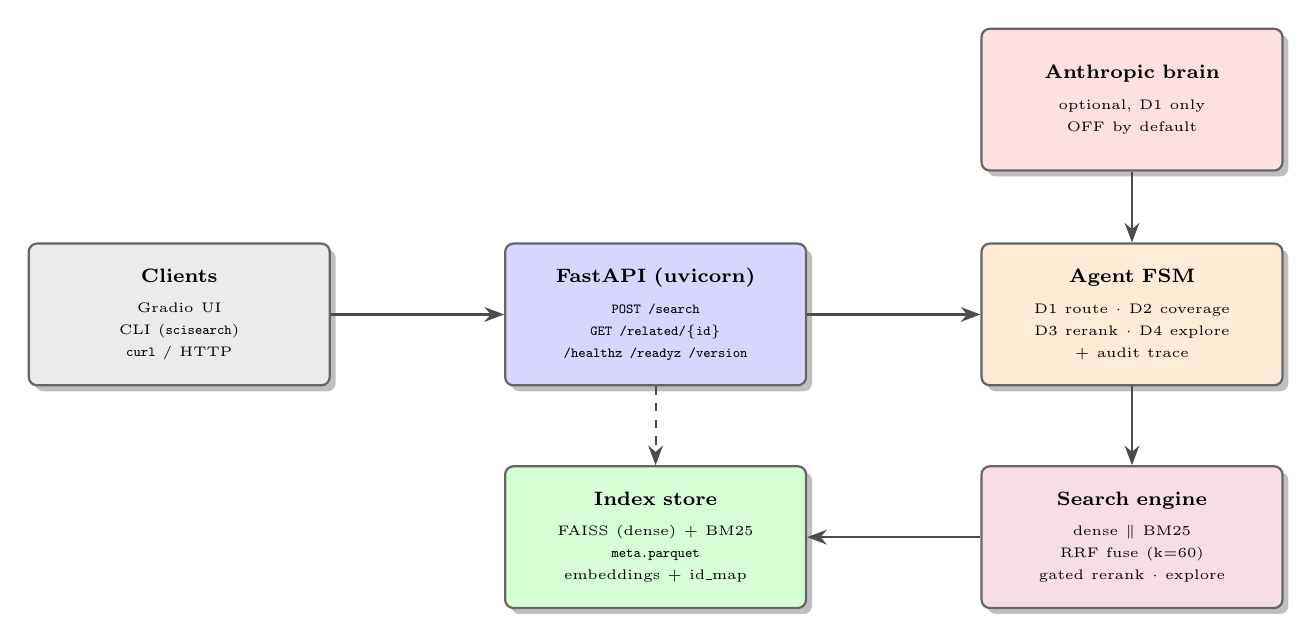
\begin{tikzpicture}[
  node distance=1.0cm and 2.2cm,
  box/.style={rectangle, draw=black!60, rounded corners=3pt, thick,
             text width=3.4cm, minimum height=1.8cm, align=center,
             inner sep=6pt, font=\scriptsize, drop shadow},
  clientbox/.style={box, fill=gray!16},
  apibox/.style={box, fill=blue!16},
  agentbox/.style={box, fill=orange!16},
  enginebox/.style={box, fill=purple!13},
  databox/.style={box, fill=green!16},
  brainbox/.style={box, fill=red!12},
  arrow/.style={-{Stealth[length=2.5mm]}, thick, color=black!70}
]

\node[clientbox] (cli) {%
  \textbf{Clients}\\[3pt]
  {\tiny Gradio UI}\\
  {\tiny CLI (\texttt{scisearch})}\\
  {\tiny \texttt{curl} / HTTP}
};
\node[apibox, right=of cli] (api) {%
  \textbf{FastAPI (uvicorn)}\\[3pt]
  {\tiny \texttt{POST /search}}\\
  {\tiny \texttt{GET /related/\{id\}}}\\
  {\tiny \texttt{/healthz /readyz /version}}
};
\node[agentbox, right=of api] (agent) {%
  \textbf{Agent FSM}\\[3pt]
  {\tiny D1 route $\cdot$ D2 coverage}\\
  {\tiny D3 rerank $\cdot$ D4 explore}\\
  {\tiny + audit trace}
};
\node[enginebox, below=1.0cm of agent] (engine) {%
  \textbf{Search engine}\\[3pt]
  {\tiny dense $\parallel$ BM25}\\
  {\tiny RRF fuse (k=60)}\\
  {\tiny gated rerank $\cdot$ explore}
};
\node[databox, below=1.0cm of api] (store) {%
  \textbf{Index store}\\[3pt]
  {\tiny FAISS (dense) + BM25}\\
  {\tiny \texttt{meta.parquet}}\\
  {\tiny embeddings + id\_map}
};
\node[brainbox, above=0.9cm of agent] (brain) {%
  \textbf{Anthropic brain}\\[3pt]
  {\tiny optional, D1 only}\\
  {\tiny OFF by default}
};

\draw[arrow] (cli.east) -- (api.west);
\draw[arrow] (api.east) -- (agent.west);
\draw[arrow] (agent.south) -- (engine.north);
\draw[arrow] (engine.west) -- (store.east);
\draw[arrow] (brain.south) -- (agent.north);
\draw[arrow, dashed] (api.south) -- (store.north);

\end{tikzpicture}%
}
\caption{Deployment architecture. All client surfaces (UI, CLI, HTTP) hit one FastAPI process that delegates to a single agent + engine (resolved via \texttt{api/dependencies.py} singletons). The engine reads a FAISS + BM25 + metadata index store. The optional Anthropic brain advises only D1 and is OFF by default, so the default configuration makes zero external calls.}
\label{fig:arch}
\end{figure}

\subsection{API Contract and Endpoints}

\begin{table}[H]
\centering
\caption{FastAPI endpoints}
\small
\begin{tabularx}{\linewidth}{@{} l l L @{}}
\toprule
\textbf{Method} & \textbf{Path} & \textbf{Description} \\
\midrule
GET & \texttt{/healthz} & Liveness -- process is up \\
GET & \texttt{/readyz} & Readiness -- FAISS index built and models loaded \\
GET & \texttt{/version} & Active model + index version (\texttt{repo@revision}) \\
POST & \texttt{/search} & Run a full exploratory search for a query \\
GET & \texttt{/related/\{paper\_id\}} & Dense nearest-neighbour rail for one paper \\
\bottomrule
\end{tabularx}
\end{table}

A \texttt{POST /search} returns a single JSON object with everything the UI needs to render:

\begin{lstlisting}[basicstyle=\ttfamily\footnotesize]
// 200 OK
{
  "results":     [ {"paper_id":"...", "title":"...", "abstract":"...",
                    "score":0.71, "field":"cs.CL", "reranked":true} ],
  "facets":      [ {"field":"cs.CL", "count":7} ],
  "clusters":    [ {"label":"passage ranking, retrieval", "members":["..."]} ],
  "suggestions": {"broaden":["..."], "narrow":["..."], "related":["..."]},
  "decisions":   [ {"point":"D1", "choice":"conceptual", "reason":"..."} ],
  "metrics":     {"latency_ms":0.0, "reranked":true}
}
\end{lstlisting}

The \texttt{decisions} field is the full agent audit trace of D1--D4 -- it is part of the returned payload, not a side-channel log, so a grader or user can inspect \emph{why} each branch fired.

\subsection{Latency, Scalability, and Graceful Degradation}

\begin{table}[H]
\centering
\caption{Latency profile}
\begin{tabular}{ll}
\toprule
\textbf{Stage} & \textbf{Cost} \\
\midrule
Hot path (dense + BM25 + RRF) & $\sim$tens of ms on a 100k--500k FAISS slice \\
Reranking (cross-encoder, gated by D3) & $+150$--$400$\,ms, only when fired \\
End-to-end & sub-second \\
\bottomrule
\end{tabular}
\end{table}

The D3 rerank gate is the key latency lever: most queries with an unambiguous top result skip the cross-encoder and stay in the tens-of-ms range. \textbf{Scalability} comes from FAISS index sharding (fan-out then RRF-merge across shards), cached embeddings (computed once, memory-mapped), and one-time model loading at startup. \textbf{Graceful degradation}: a numpy brute-force store substitutes for FAISS, a TF-IDF retriever for the dense slot, an identity reranker for the cross-encoder, and a built-in $\sim$40-paper corpus for the dataset -- so the full pipeline runs offline with no GPU and no network.

\subsection{Model Versioning}

Versioning is handled by the model registry (\texttt{models/model\_registry.py}): \texttt{model\_meta.json} records each trained build's metadata, a \texttt{latest} pointer selects the active build, and models are pinned by \texttt{repo@revision}. The \texttt{/version} endpoint reports the active model and index versions, so every served response is traceable to an exact model build. Re-embedding builds a new index version side-by-side (blue/green); the \texttt{latest} pointer cuts over atomically and rollback is a pointer move.

% ============================================================
\section{Agentic AI Component}
% ============================================================

\subsection{Agent Architecture}

The agent is the mandatory agentic component that turns a flat retrieval pipeline into an \emph{exploratory} search experience. It is a \textbf{deterministic finite-state machine (FSM)} with \textbf{four decision points (D1--D4)} acting on intermediate outputs, plus an \emph{optional} LLM query-understanding brain at D1 and a \textbf{full audit trace} of every decision. The agent does not free-roam: every transition is governed by explicit thresholds over a shared \texttt{JobState}, so the same query + same index + brain disabled always produces an identical path (reproducible, debuggable, gradeable). The optional Anthropic brain is OFF by default -- the agent incurs \textbf{zero paid API calls} in the default configuration -- and even when enabled it only \emph{advises} D1, validating its output and falling back to rules on any failure.

The pipeline encodes the classic exploratory-search loop: \textbf{understand} (D1) $\rightarrow$ \textbf{retrieve + RRF fuse} (D2 coverage gate $\rightarrow$ expand) $\rightarrow$ \textbf{rerank} (D3 gate) $\rightarrow$ \textbf{explore} (D4: facets + clusters + related).

\begin{figure}[H]
\centering
\resizebox{0.92\linewidth}{!}{%
\begin{tikzpicture}[
  node distance=0.34cm,
  step/.style={rectangle, draw=black!60, rounded corners=2pt, thick,
              text width=12.5cm, inner sep=5pt, minimum height=0.7cm,
              align=center, font=\footnotesize},
  s0/.style={step, fill=gray!15},
  dec/.style={step, fill=red!12},
  ret/.style={step, fill=blue!15},
  rer/.style={step, fill=purple!15},
  exp/.style={step, fill=green!15},
  out/.style={step, fill=green!10},
  arrow/.style={-{Stealth[length=2mm]}, thick}
]

\node[s0] (entry) {\textbf{ENTRY}: raw query $\rightarrow$ \texttt{JobState}};
\node[dec, below=of entry] (d1) {\textbf{D1 -- Query-type routing} (\textit{tool\_understand} + optional brain): intent $\in$ \{keyword, conceptual, hybrid\} + filters (field, year) $\rightarrow$ biases RRF fusion};
\node[ret, below=of d1] (s1) {\textbf{RETRIEVE + FUSE} (\textit{tool\_retrieve}): dense $\parallel$ BM25 $\rightarrow$ \texttt{rrf\_fuse(k=60)} $\rightarrow$ \texttt{fused\_ranking}, \texttt{top\_raw\_score}, \texttt{n\_results}};
\node[dec, below=of s1] (d2) {\textbf{D2 -- Coverage gate} (\textit{decision-making}): if \texttt{n\_results} too few \textbf{or} \texttt{top\_raw\_score} $<$ threshold $\rightarrow$ \texttt{expand\_query} (abbrev map + PRF) + re-retrieve (loop guard); else \texttt{coverage\_ok}};
\node[dec, below=of d2] (d3) {\textbf{D3 -- Rerank gate} (\textit{decision-making}): if \texttt{head\_margin} small/ambiguous $\rightarrow$ \texttt{rerank}; else \texttt{skip\_rerank} (saves $+150$--$400$\,ms)};
\node[rer, below=of d3] (s2) {\textbf{RERANK} (\textit{tool\_rerank}, gated): \texttt{cross-encoder/ms-marco-MiniLM-L-6-v2} re-scores top-k $\rightarrow$ \texttt{final\_ranking} (identity fallback if absent)};
\node[exp, below=of s2] (d4) {\textbf{D4 -- Exploration strategy} (\textit{multi-step reasoning} + \textit{tool\_explore}): facets + KMeans/TF-IDF clusters + related NN; diversity $\rightarrow$ \texttt{broaden} / \texttt{narrow} / \texttt{related}};
\node[out, below=of d4] (s4) {\textbf{PRESENT}: \{results, facets, clusters, suggestions, \textbf{decisions[]} (audit trace), metrics\}};

\foreach \a/\b in {entry/d1, d1/s1, s1/d2, d2/d3, d3/s2, s2/d4, d4/s4}
  \draw[arrow] (\a) -- (\b);

\end{tikzpicture}%
}
\caption{The deterministic FSM with four decision points. D1 and D4 involve multi-step reasoning / understanding; D2 and D3 are decision-making gates over intermediate outputs; tools (understand, retrieve, rerank, explore) are invoked at each stage. Every decision is recorded in \texttt{decisions[]}.}
\label{fig:agent}
\end{figure}

\subsection{The Four Decision Points}

\begin{table}[H]
\centering
\caption{Decision points D1--D4 (named exactly as in \texttt{docs/agent\_architecture.md}). Each is a pure threshold function in \texttt{agent/policy.py}.}
\small
\begin{tabularx}{\linewidth}{@{} l l L @{}}
\toprule
\textbf{ID} & \textbf{Decision} & \textbf{Inputs $\rightarrow$ branches / effect} \\
\midrule
D1 & Query-type routing & \texttt{raw\_query} (length, wh-words), optional LLM hint $\rightarrow$ \texttt{keyword} $|$ \texttt{conceptual} $|$ \texttt{hybrid} + filters; biases RRF by duplicating the preferred ranking \\
D2 & Coverage gate & \texttt{n\_results}, \texttt{top\_raw\_score} $\rightarrow$ \texttt{coverage\_ok} $|$ \texttt{expand\_and\_retry} (abbrev map + PRF, then re-retrieve). Backstops the zero-result rate $<2\%$ \\
D3 & Rerank gate & \texttt{head\_margin} (score gap at the head) $\rightarrow$ \texttt{rerank} (ambiguous head) $|$ \texttt{skip\_rerank} (decisive head). Saves $+150$--$400$\,ms \\
D4 & Exploration strategy & \texttt{final\_ranking} + diversity (\#fields / cluster count) $\rightarrow$ suggestion mode \texttt{broaden} $|$ \texttt{narrow} $|$ \texttt{related}; emits facets + clusters + related \\
\bottomrule
\end{tabularx}
\end{table}

\paragraph{Tool contracts.} The FSM driver calls four typed, side-effect-free tools: \texttt{tool\_understand} (intent + filters), \texttt{tool\_retrieve} (dense $\parallel$ BM25 $\rightarrow$ RRF), \texttt{tool\_rerank} (gated cross-encoder), and \texttt{tool\_explore} (facets, clusters, related, suggestions). Graceful degradation is built into the contracts: when \texttt{torch}/network are absent, the retriever slot is filled by a TF-IDF retriever, the reranker degrades to identity, and retrieval runs over the built-in mini-corpus -- so the agent always completes end-to-end offline.

\paragraph{Optional LLM brain (D1 only).} The Anthropic brain (\texttt{llm\_orchestrator.py}) is a thin advisor wired only into D1 query understanding. It produces a structured understanding (intent + filters), the output is schema-validated, and on any validation failure -- or when disabled -- the agent falls back to the deterministic rule-based D1. It is OFF by default, guaranteeing zero paid API usage and full offline operation; it never replaces the deterministic D2--D4 gates.

\subsection{Example Interaction (Validated Offline)}

\begin{lstlisting}
# Worked example -- a conceptual query
Input: "dense passage retrieval"
  D1 understand : concept phrase, no field filter -> intent = CONCEPTUAL
                  (fusion will up-weight the dense ranking)
  Retrieve+RRF  : dense (bge-small, fine-tuned) || BM25 -> rrf_fuse(k=60),
                  dense ranking duplicated to honor the conceptual bias
  D2 coverage   : plenty of results + strong head similarity -> coverage_ok
                  (no expansion needed)
  D3 rerank     : head is close/ambiguous (small head_margin) -> RERANK
                  cross-encoder ms-marco-MiniLM-L-6-v2 re-scores top-k
  D4 explore    : KMeans/TF-IDF clusters + arXiv-field facets +
                  dense-NN related rail -> suggestion = related
Outcome: the Dense Passage Retrieval paper ranks #1; all four decisions
         fire and are recorded in decisions[]; the response carries
         facets + topic clusters + related rails + the suggestion strip.
\end{lstlisting}

This trace was validated offline on the built-in mini-corpus (TF-IDF retriever + identity reranker), confirming correct intent routing and that all four decision points fire with a full audit trace.

% ============================================================
\section{Continual Learning \& Monitoring}
\label{sec:continual}
% ============================================================

\subsection{New-Data Collection}

Two decoupled streams feed the continual-learning loop: one keeps the \textbf{index} current, the other keeps the \textbf{ranker} current.
\begin{itemize}\setlength\itemsep{0.15em}
  \item \textbf{Incremental ingestion (index freshness)}: harvest new arXiv records (same schema), dedup by \texttt{id} (arXiv ids are stable), embed \texttt{title+abstract} with the \emph{current registered retriever} (so new vectors share the live embedding space), and append to FAISS + BM25 + facet metadata. A full re-embed is only needed when the retriever itself is upgraded.
  \item \textbf{Feedback harvesting (training pairs)}: each \texttt{POST /search} returns results the UI logs as opened/relevant, yielding implicit \texttt{(query, clicked\_paper)} pairs -- true positives reflecting real intent -- that complement the generated cold-start pairs. Privacy constraint: minimize raw-query retention; prefer the \texttt{(query\_id, paper\_id, rank)} tuple over verbatim text.
\end{itemize}

\subsection{Retraining and Rollout}

Retraining is \textbf{periodic} and \textbf{event-driven} (fired when monitoring crosses a threshold). The recipe is unchanged from initial training (MNRL, large in-batch-negative batches, 1--3 epochs, anti-overfitting via dedup). Every candidate must pass an \textbf{offline gate} -- beat \emph{both} BM25 and the zero-shot base on nDCG@10 (and not regress on conceptual queries) -- before any live traffic, then prove out on a \textbf{canary / AB} slice against the monitoring metrics before the \texttt{latest} pointer advances. Either way the decision is reversible by moving the registry pointer (blue/green re-embed for a new embedding space).

\subsection{Monitoring Metrics and Drift}

\begin{table}[H]
\centering
\caption{Monitoring dashboard (\texttt{src/scisearch/monitoring/drift\_report.py})}
\small
\begin{tabularx}{\linewidth}{@{} l L @{}}
\toprule
\textbf{Metric} & \textbf{Why it matters / target} \\
\midrule
Zero-result rate & Business target $<2\%$; the D2 coverage gate is the backstop. A rise means index/expansion is failing. \\
Intent mix (D1) & Detects query-distribution shift; a swing changes which retriever (BM25 vs.\ dense) carries the load. \\
Latency & Hot path tens of ms; gated rerank adds $+150$--$400$\,ms; target sub-second end-to-end. \\
nDCG@10 on a golden set & Headline quality signal re-scored every cycle; a sustained drop is the primary degradation trigger. \\
Click-through (CTR) & Live relevance proxy; feeds the feedback harvester and the AB comparison. \\
\bottomrule
\end{tabularx}
\end{table}

A fixed \textbf{golden query set} re-scored each cycle isolates model/index regressions from genuine user-behaviour changes. The drift report flags threshold breaches (quality, behaviour, performance) and, when a breach is sustained, signals the retraining trigger / canary rollback.

% ============================================================
\section{Data Privacy \& Model Robustness}
% ============================================================

\subsection{Privacy: the Query is the Sensitive Asset}

The corpus is \emph{public} (\texttt{gfissore/arxiv-abstracts-2021}, CC0; author names are already-published bibliographic data -- no PII to scrub). The asymmetry that drives the whole design is that the \textbf{query} can reveal a research direction or unfiled IP. Controls:
\begin{itemize}\setlength\itemsep{0.15em}
  \item \textbf{Minimize retention}: keep the raw query request-scoped; hash/redact it in traces; put a TTL on any query log.
  \item \textbf{No egress}: the entire hot path runs locally (\texttt{faiss-cpu}, \texttt{scikit-learn}, \texttt{numpy}); the optional LLM brain is OFF by default $\Rightarrow$ \textbf{zero paid API calls and zero query egress} in the default configuration. An org with confidential research can run fully on-prem.
  \item \textbf{Aggregated telemetry}: success metrics (zero-result rate, exploration depth) are aggregate counters, not query text.
\end{itemize}

\subsection{Robustness}

Robustness is enforced by the deterministic FSM (\texttt{agent/policy.py}) and query expansion (\texttt{search/expand.py}). Hard inputs (out-of-domain, garbled, very short) share a symptom -- weak retrieval signal -- which the \textbf{D2 coverage gate} catches: too few hits or low top-similarity $\rightarrow$ expand (abbreviation map + pseudo-relevance feedback) and re-retrieve. This is the mechanism behind the zero-result-rate $<2\%$ target.

\begin{table}[H]
\centering
\caption{Known failure cases and honest handling}
\small
\begin{tabularx}{\linewidth}{@{} l L @{}}
\toprule
\textbf{Failure case} & \textbf{Mitigation} \\
\midrule
Topic absent from corpus & D2 expands; if still weak, D4 surfaces \texttt{broaden} suggestions and low scores -- relevance is never fabricated \\
Ambiguous acronym & Best-effort abbreviation map; D4 topic clustering splits competing senses into distinct clusters \\
Non-English query & English-centric retriever; recall degrades; documented limitation, not silently masked (scores read low) \\
Post-2021 recency & Snapshot cutoff documented; incremental-update plan; out of scope for the static index \\
\bottomrule
\end{tabularx}
\end{table}

\paragraph{Graceful degradation.} Each component has a self-contained fallback (TF-IDF retriever, numpy store, identity reranker, built-in mini-corpus, rule-based D1), so the agent runs end-to-end offline -- degradation is in \emph{quality}, never in \emph{availability}.

\paragraph{Over-trust mitigation.} The subtlest risk is human: users treating the top result as exhaustive/authoritative. The presentation layer counters this by always \textbf{showing scores}, exposing \textbf{diversity} (facets + topic clusters), surfacing \textbf{broaden} suggestions, and reporting \textbf{Recall@k} alongside nDCG/MRR so coverage -- not just top-1 precision -- is visible.

% ============================================================
\section{Project Management}
% ============================================================

This project was completed \textit{individually}. The work is organised into eight phases, each with a concrete exit artifact; the headline gate is the fine-tuned retriever beating \emph{both} BM25 and the zero-shot base encoder on nDCG@10.

\begin{table}[H]
\centering
\caption{Project plan -- phases, milestones, and indicative solo timeline}
\small
\begin{tabularx}{\linewidth}{@{} c l L c @{}}
\toprule
\textbf{\#} & \textbf{Phase} & \textbf{Exit artifact / milestone} & \textbf{Cum.\ days} \\
\midrule
0 & Research \& design & This plan + verified model/dataset ids in \texttt{config.py} & D2 \\
1 & Corpus + pairs + BM25 & Indexed slice + pair set + BM25 baseline nDCG@10 & D5 \\
2 & Retriever fine-tune & Fine-tuned checkpoint + \texttt{model\_meta.json} & D7 \\
3 & Hybrid + rerank + facets & Engine beats BM25 \emph{and} zero-shot on nDCG@10 (gate) & D10 \\
4 & Agent & FSM D1--D4 runs end-to-end with full audit trace & D12 \\
5 & Deployment & FastAPI + Gradio + CLI + Docker; sub-second hot path & D14 \\
6 & Evaluation & nDCG@10 / Recall@\{1,5,10\} / MRR@10 + latency report & D16 \\
7 & Docs \& report & README, docs, auto-generated \texttt{report.pdf} + \texttt{slides.pptx} & D18 \\
\bottomrule
\end{tabularx}
\end{table}

The plan maps onto simulated cross-functional roles (ML/IR Engineer, Data Engineer, Search/Backend Engineer, Agent Engineer, Frontend Engineer, QA Engineer, Project Manager), each owning a package boundary that already exists -- so the solo build translates directly to parallel team workstreams once Phase 1 lands. The \texttt{scisearch} CLI is the integration seam between roles.

\textbf{Scaling reflection}: A real team would add a CI eval gate (a PR cannot merge if nDCG@10 regresses vs.\ the registered baseline), a promote/rollback model-registry workflow, a sharded FAISS indexing pipeline for millions of papers, a click/dwell relevance-feedback loop, latency/error SLOs with on-call, and scheduled continual ingestion to kill the stale-index risk.

% ============================================================
\section{Ethics \& Responsible AI}
% ============================================================

\textbf{Guiding principle:} the system presents a ranked, explorable \emph{sample} of the literature -- never an exhaustive or authoritative verdict.

\subsection{Who Benefits}
Researchers (faster time-to-first-relevant-result; semantic recall surfaces concept matches BM25 is blind to), students/newcomers (facets + clusters map an unfamiliar area), and R\&D teams (broad discovery with an on-prem option to keep search direction private).

\subsection{Who Could Be Harmed}
Users who over-rely on the ranking (risking missed work and citation bias); authors whose papers are systematically under-ranked (niche fields, unusual phrasing); and, via dual-use surfacing, society at large -- though the system indexes only \textbf{public, already-published} arXiv papers and creates no new capability, only easier discovery of what is already public.

\subsection{Bias \& Fairness}
The system inherits and can amplify biases, documented rather than hidden:
\begin{itemize}\setlength\itemsep{0.15em}
  \item \textbf{Coverage bias}: arXiv-only, English, 2021 cutoff -- bounds what the system can \emph{ever} return.
  \item \textbf{Ranking bias}: the dense encoder rewards mainstream phrasing; niche fields may be under-ranked.
\end{itemize}
\textbf{Mitigations}: hybrid retrieval (RRF keeps BM25's exact-term recall so niche papers can still surface); \textbf{Recall@\{1,5,10\}} reported alongside nDCG@10 so under-ranking is measurable; the D2 coverage gate + query expansion; and faceting/clustering that make the field/topic distribution explicit. These make bias \emph{observable and partially correctable}, not eliminated.

\subsection{Explainability and Misuse Safeguards}
The \texttt{/search} response and Gradio UI expose five explanation surfaces -- relevance scores, facets, topic clusters, the D1--D4 decision log, and broaden/narrow/related suggestions -- so a non-technical user can understand \emph{why} they see what they see and \emph{what they are not} seeing. Safeguards: public-papers-only indexing; query privacy (minimized retention; on-prem option); transparency about coverage/recency; and no paid LLM by default (the optional brain is OFF and validates against / falls back to deterministic rules, so no query text is sent to a third-party API unless explicitly enabled).

% ============================================================
\section{Conclusion \& Future Work}
% ============================================================

\subsection{Summary}
\begin{itemize}\setlength\itemsep{0.15em}
  \item Complete end-to-end exploratory-search system: data $\rightarrow$ training $\rightarrow$ hybrid engine $\rightarrow$ agent $\rightarrow$ deployment $\rightarrow$ monitoring.
  \item Trainable core: a fine-tuned \texttt{BAAI/bge-small-en-v1.5} bi-encoder (MNRL, in-batch negatives), required to beat \emph{both} BM25 and the zero-shot base on nDCG@10 -- with the largest margin on conceptual queries.
  \item Hybrid stack: dense $\parallel$ BM25 $\rightarrow$ RRF fusion ($k=60$) $\rightarrow$ gated cross-encoder rerank; an exploration layer of facets, KMeans/TF-IDF clusters, related rails, and broaden/narrow guidance.
  \item Deterministic 4-decision FSM agent (D1 routing, D2 coverage gate, D3 rerank gate, D4 exploration) with a full audit trace and an optional, OFF-by-default Anthropic brain at D1.
  \item Verified offline end-to-end (built-in corpus, no GPU/network): all four decisions fire, intent routing is correct (DPR query $\rightarrow$ \#1), facets + clusters produced; the full IR numbers are produced by the real Colab/H100 run.
  \item Deployable via FastAPI + Gradio + CLI + Docker + HF Space app; license-clean (CC0 corpus, MIT/Apache models, MIT code).
\end{itemize}

\subsection{Future Work}
\begin{enumerate}\setlength\itemsep{0.15em}
  \item \textbf{Hard negatives}: BM25-mined hard negatives on top of in-batch negatives (the biggest lever after the loss).
  \item \textbf{Larger/domain encoders}: ablate \texttt{malteos/scincl} / \texttt{allenai/specter2\_base} (768-dim) for the related-work NN rail.
  \item \textbf{Continual ingestion}: scheduled harvest of post-2021 arXiv papers to kill the stale-index risk.
  \item \textbf{Relevance-feedback loop}: capture click/dwell signals $\rightarrow$ harvested \texttt{(query, clicked\_paper)} pairs $\rightarrow$ periodic re-fine-tune.
  \item \textbf{Sharded indexing}: FAISS sharding + distributed embedding jobs to scale to the full 2.0M corpus and beyond.
  \item \textbf{Monitoring}: a live drift dashboard (nDCG@10 on the golden set, zero-result rate, intent mix, latency, CTR) with canary A/B rollout.
\end{enumerate}

% ============================================================
\newpage
\begin{thebibliography}{9}

\bibitem{bge} Xiao, S., Liu, Z., Zhang, P., \& Muennighoff, N. (2023). C-Pack: Packed Resources For General Chinese Embeddings (BGE). \url{https://huggingface.co/BAAI/bge-small-en-v1.5}

\bibitem{sbert} Reimers, N., \& Gurevych, I. (2019). Sentence-BERT: Sentence Embeddings using Siamese BERT-Networks. \textit{EMNLP 2019}.

\bibitem{mnrl} Henderson, M., et al. (2017). Efficient Natural Language Response Suggestion (MultipleNegativesRankingLoss / in-batch negatives). \textit{arXiv:1705.00652}.

\bibitem{minilm} Wang, W., et al. (2020). MiniLM: Deep Self-Attention Distillation. \textit{NeurIPS 2020}. (\texttt{all-MiniLM-L6-v2}).

\bibitem{dpr} Karpukhin, V., et al. (2020). Dense Passage Retrieval for Open-Domain Question Answering. \textit{EMNLP 2020}.

\bibitem{rrf} Cormack, G.\,V., Clarke, C.\,L.\,A., \& B\"uttcher, S. (2009). Reciprocal Rank Fusion outperforms Condorcet and individual Rank Learning Methods. \textit{SIGIR 2009}.

\bibitem{bm25} Robertson, S., \& Zaragoza, H. (2009). The Probabilistic Relevance Framework: BM25 and Beyond. \textit{Foundations and Trends in IR}.

\bibitem{scifact} Wadden, D., et al. (2020). Fact or Fiction: Verifying Scientific Claims (SciFact). \textit{EMNLP 2020}. (\texttt{BeIR/scifact}).

\bibitem{beir} Thakur, N., et al. (2021). BEIR: A Heterogeneous Benchmark for Zero-shot Evaluation of Information Retrieval Models. \textit{NeurIPS 2021}.

\bibitem{faiss} Johnson, J., Douze, M., \& J\'egou, H. (2019). Billion-scale similarity search with GPUs (FAISS). \textit{IEEE Transactions on Big Data}.

\bibitem{arxivds} Fissore, G. \textit{arXiv Abstracts 2021}. Hugging Face Datasets. \url{https://huggingface.co/datasets/gfissore/arxiv-abstracts-2021}

\bibitem{msmarco} Nogueira, R., \& Cho, K. (2019). Passage Re-ranking with BERT. (\texttt{cross-encoder/ms-marco-MiniLM-L-6-v2}).

\bibitem{nlpkg} NLP-KG Team. \textit{NLP-KG-WebApp}. \url{https://github.com/NLP-Knowledge-Graph/NLP-KG-WebApp}

\end{thebibliography}

\end{document}
